\section{Appendix}
\renewcommand{\thesubsection}{\textcolor{black}{\textbf{\Alph{subsection}}}}
\subsection{Table of decomposed metrics}\label{decomposed_metrics}
\begin{table}[H]
\begin{tabular}{l l l}
\hline 
\textbf{Disparity} \\
\hline 
\text { II-D } &=& $\frac{1}{|\mathcal{D}|} \frac{1}{|\mathcal{U}|} \sum_{j=1}^{|\mathcal{D}|} \sum_{i=1}^{|\mathcal{U}|} \mathrm{E}_{i j}^{\delta_{i j}^2}$ 
\\
\text { IG-D } &=& $\frac{1}{\left|\mathcal{G}_d\right|} \frac{1}{|\mathcal{U}|} \sum_{D \in \mathcal{G}_d} \sum_{i=1}^{|\mathcal{U}|}\left(\sum_{j=1}^{|D|} p\left(D_j \mid D\right) \mathrm{E}^\delta{ }_{i j}\right)^2 \quad \quad$ \\
\text { GI-D } &=& $\frac{1}{|\mathcal{D}|} \frac{1}{\left|\mathcal{G}_u\right|} \sum_{j=1}^{|\mathcal{D}|} \sum_{U \in \mathcal{G}_u}\left(\sum_{i=1}^{|U|} p\left(U_i \mid U\right) \mathbf{E}^\delta{ }_{i j}\right)^2 \quad \quad $ \\
\text { GG-D } &=& $\frac{1}{\left|\mathcal{G}_d\right|} \frac{1}{\left|\mathcal{G}_u\right|} \sum_{D \in \mathcal{G}_d} \sum_{U \in \mathcal{G}_u}\left(\sum_{j=1}^{|D|} \sum_{i=1}^{|U|} p\left(D_j \mid D\right) p\left(U_i \mid U\right) \mathbf{E}^\delta{ }_{i j}\right)^2 \quad$ \\
\text { AI-D } &=& $\sum_{j=1}^{|\mathcal{D}|}\left(\sum_{i=1}^{|\mathcal{U}|} p\left(\mathcal{U}_i\right) \mathrm{E}^\delta{ }_{i j}\right)^2 \quad \quad $ \\
\text { AG-D } &=& $\frac{1}{\left|\mathcal{G}_d\right|} \sum_{D \in \mathcal{G}_d}\left(\sum_{j=1}^{|D|} \sum_{i=1}^{|\mathcal{U}|} p\left(D_j \mid D\right) p\left(\mathcal{U}_i\right) \mathrm{E}^\delta{ }_{i j}\right)^2 \quad $\\
\hline

\textbf{Relevance} \\
\hline
\text { II-R } &=& $\frac{1}{|\mathcal{D}|} \frac{1}{|\mathcal{U}|} \sum_{j=1}^{|\mathcal{D}|} \sum_{i=1}^{|\mathcal{U}|} 2 \mathrm{E}^\delta{ }_{i j} \mathrm{E}^{\Delta}{ }_{i j}$ \\
\text { IG-R } &=& $\frac{1}{\left|\mathcal{G}_d\right|} \frac{1}{|\mathcal{U}|} \sum_{D \in \mathcal{G}_d} \sum_{i=1}^{|\mathcal{U}|}\left(\sum_{j=1}^{|D|} 2 p\left(D_j \mid D\right) \mathrm{E}^\delta{ }_{i j} \mathrm{E}^{\Delta}{ }_{i j}\right)^2$ \\
\text { GI-R } &=& $\frac{1}{|\mathcal{D}|} \frac{1}{\left|\mathcal{G}_u\right|} \sum_{j=1}^{|\mathcal{D}|} \sum_{U \in \mathcal{G}_u}\left(\sum_{i=1}^{|U|} 2 p\left(U_i \mid U\right) \mathrm{E}^\delta{ }_{i j} \mathrm{E}^{\Delta}{ }_{i j}\right)^2$  \\
\text { GG-R } &=& $\frac{1}{\left|\mathcal{G}_d\right|} \frac{1}{\left|\mathcal{G}_u\right|} \sum_{D \in \mathcal{G}_d} \sum_{U \in \mathcal{G}_u}\left(\sum_{j=1}^{|D|} \sum_{i=1}^{|U|} 2 p\left(D_j \mid D\right) p\left(U_i \mid U\right) \mathrm{E}^\delta{ }_{i j} \mathrm{E}^{\Delta}{ }_{i j}\right)^2 $\\
\text { AI-R } &=& $\sum_{j=1}^{|\mathcal{D}|}\left(\sum_{i=1}^{|\mathcal{U}|} 2 p\left(\mathcal{U}_i\right) \mathrm{E}^\delta{ }_{i j} \mathrm{E}^{\Delta}{ }_{i j}\right)^2$  \\
\text { AG-R } &=& $\frac{1}{\left|\mathcal{G}_d\right|} \sum_{D \in \mathcal{G}_d}\left(\sum_{j=1}^{|D|} \sum_{i=1}^{|\mathcal{U}|} 2 p\left(D_j \mid D\right) p\left(\mathcal{U}_i\right) \mathrm{E}^\delta{ }_{i j} \mathrm{E}^{\Delta}{ }_{i j}\right)^2 $ \\
\hline
\end{tabular}
\caption{\label{metric_decomp}
Decomposition of each JME-fairness metric into their disparity and relevance components, where $\mathrm{E}^\delta{ }_{i j} = \mathrm{E}_{i j} - \mathrm{E}^\sim_{i j}$ and $\mathrm{E}^{\Delta}{ }_{i j} = \mathrm{E}^*_{i j} - \mathrm{E}^\sim_{i j}$
}
\end{table}

\renewcommand{\thesubsection}{\textbf{\textcolor{black}{B}}}
\subsection{AUC table: Trapezoidal Rule} 
\begin{table}[H]
\centering
\begin{tabular}{lllllll}
\hline
\textbf{Model} & \textbf{II} & \textbf{IG} & \textbf{GI} & \textbf{GG} & \textbf{AI} & \textbf{AG} \\
\hline
BPRMF  &  \ \underline{0.6336} & \textbf{0.5378} & 0.3555 &  0.3790  &  0.3324  & 0.3051  \\ 
LDA  &  0.5567 & 0.509  & 0.4671  &  0.1877  & 0.4148   & 0.1799 \\ 
PureSVD  &  0.5691  &  0.3239  &  \underline{0.5733}  & \underline{0.5048}  & \underline{0.4995}  &  \underline{0.3853}  \\ 
SLIM  &  \textbf{0.6540}  &  0.5129  &  \textbf{0.6141}  &  \textbf{0.5338}  &  \textbf{0.6141}  &  \textbf{0.5383}  \\ 
WRMF  &  0.5901  &  \underline{0.5171}  &  0.2826  &  0.334  &  0.2194  &  0.2219  \\ 
\hline
\end{tabular}
\caption{\label{our_auc}
The AUC of the disparity-relevance trade-off curves for different models across the six different fairness dimensions calculated with the trapezoidal rule. Bold text indicates the highest value in each column, and the second highest value is underlined. 
}
\end{table}

\renewcommand{\thesubsection}{\textbf{\textcolor{black}{C}}}
\subsection{Occupation as group attribute: Kendall rank correlation} \label{occupation_kendall}
\begin{figure}[H]
    \centering
    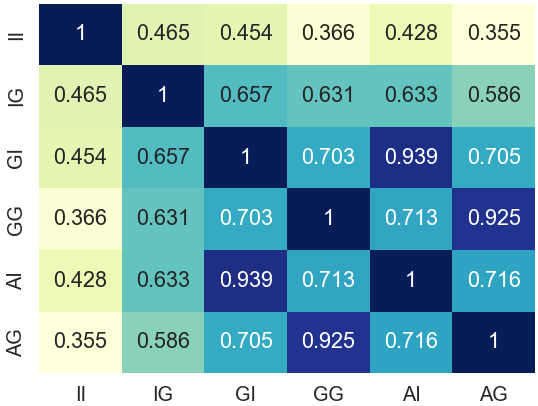
\includegraphics[width=0.32\textwidth]{Figures/Figure_4_Occupation_0.png}
    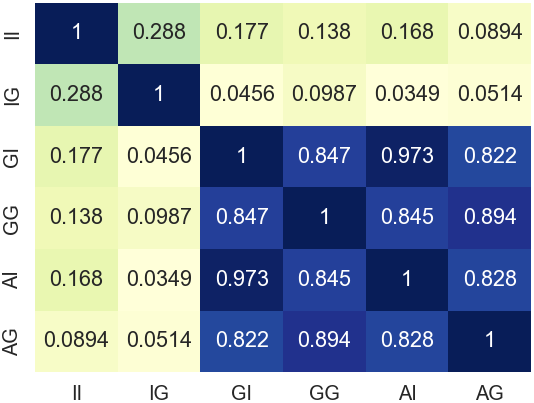
\includegraphics[width=0.32\textwidth]{Figures/Figure_4_Occupation_1.png} 
    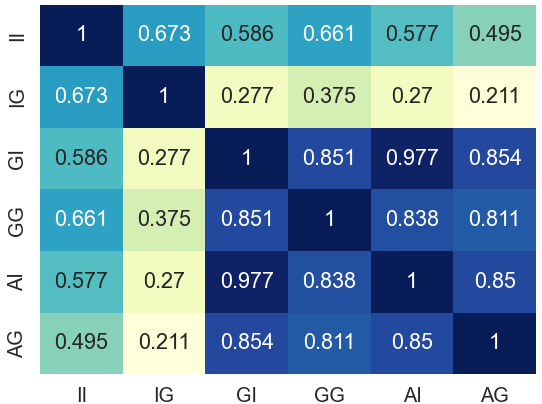
\includegraphics[width=0.32\textwidth]{Figures/Figure_4_Occupation_2.png}
    \caption{The Kendall rank correlation between the six JMEF metrics and their two components with occupation as user attributes. From the left to the right column, we respectively find the heatmaps for the fairness, disparity, and relevance components.}
    \label{occ_kendall}
\end{figure}


\renewcommand{\thesubsection}{\textbf{\textcolor{black}{D}}}
\subsection{Table of code issues} \label{code_issues}

{\centering
\begin{tabular}{p{0.5\linewidth} | p{0.5\linewidth}}
 \emph{Issue} & \emph{Provided solution} \\ \hline \hline
 The folder in which the results from running the main program are saved was missing and was not created during runtime. & Restructured codebase with the required missing folder.    \\ \hline 
 No environment to run the experiments was provided. &  Creation of an environment that is available in our repository.  \\ \hline 
 Bug in the code collocating the users into age groups was not correctly allocating them to their corresponding groups.  & Reformed code for the corresponding function. \\ \hline 
 Missing code for the calculation of the AUC used in one of the metric decomposition experiments. & Inclusion of a new function for this purpose.\\ \hline 
 The code used to plot the figures shown in the paper, as well as the heatmaps, was missing. & Creation of new functions to plot and save the results of the experiments in an image format. \\ \hline 
 The code was largely uncommented and thus difficult to follow and understand. & We added comprehensive comments, separated large functions into smaller ones, and reformed the structure of the codebase to make it easier to interpret and debug. \\ \hline
\end{tabular}\par }

\renewcommand{\thesubsection}{\textbf{\textcolor{black}{E}}}
\subsection{Figures of the results in the original paper} \label{og_results}
\begin{figure}[H]
    \centering
    \includegraphics[width=1\textwidth, height = 185pt]{Figures/og_fig2.png}
    \caption{Results for the Behavior of JME-fairness metrics for a stochastic ranking policy, generated by randomizing the BPRMF model using Placket-Luce on the MovieLens1M dataset, as shown in the paper. It corresponds to Figure \ref{fig2} of this document.}
    \label{fig: og_fig2}
\end{figure}
\begin{figure}[H]
    \centering
    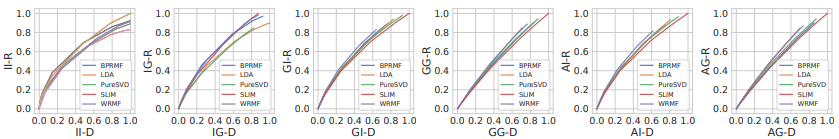
\includegraphics[width=1\textwidth, height=75pt]{Figures/og_fig3.png}
    \caption{Curves for disparity-relevance trade-off across the six different fairness dimensions, introducing different levels of stochasticity on top of the static rankings from six recommendation models, as shown in the paper. It corresponds to Figure \ref{dr_tradeoff} of this document.}
    \label{fig: og_fig3}
\end{figure}
\begin{figure}[H]
    \centering
    \includegraphics[width=1\textwidth, height=450pt]{Figures/og_fig4.png}
    \caption{The Kendall rank correlation between different metrics and their disparity and relevance across six different fairness dimensions, as shown in the paper. It corresponds to Figure \ref{kendall} of this document.}
    \label{fig: og_fig4}
\end{figure}
\begin{table}[H]
{\centering
\begin{tabular}{lllllll}
\hline
\textbf{Model} & \textbf{II} & \textbf{IG} & \textbf{GI} & \textbf{GG} & \textbf{AI} & \textbf{AG} \\
\hline
BPRMF  &  \underline{0.6331}  &  \textbf{0.4774}  &  0.2904  &  0.2953  &  0.2712  &  0.2814  \\ 
LDA  &  0.5664  &  0.4088  &  0.2837  &  \underline{0.3164}  &  0.2687  &  \underline{0.3115}  \\ 
PureSVD  &  0.5830  &  0.4102  &  \underline{0.2921}  &  0.3030  &  \underline{0.2755}  &  0.2942  \\ 
SLIM  &  \textbf{0.6408}  &  0.4654  &  0.2776  &  0.2851  &  0.2605 &  0.2752  \\ 
WRMF  &  0.5996  &  \underline{0.4769}  &  \textbf{0.3135}  &  \textbf{0.3186}  &  \textbf{0.2957}  &  \textbf{0.3139}  \\ 
\hline
\end{tabular}\par }
\caption{\label{original_auc}
The AUC of the disparity-relevance trade-off curves for different models across the six different fairness dimensions, as shown in the paper. Bold text indicates the highest value in each column, and the second highest value is underlined. 
}
\end{table}

\renewcommand{\thesubsection}{\textbf{\textcolor{black}{F}}}
\subsection{Hyperparameter sweep} \label{paramter_sweep}
\begin{figure}[H]
    \centering
    \begin{subfigure}{\textwidth}
        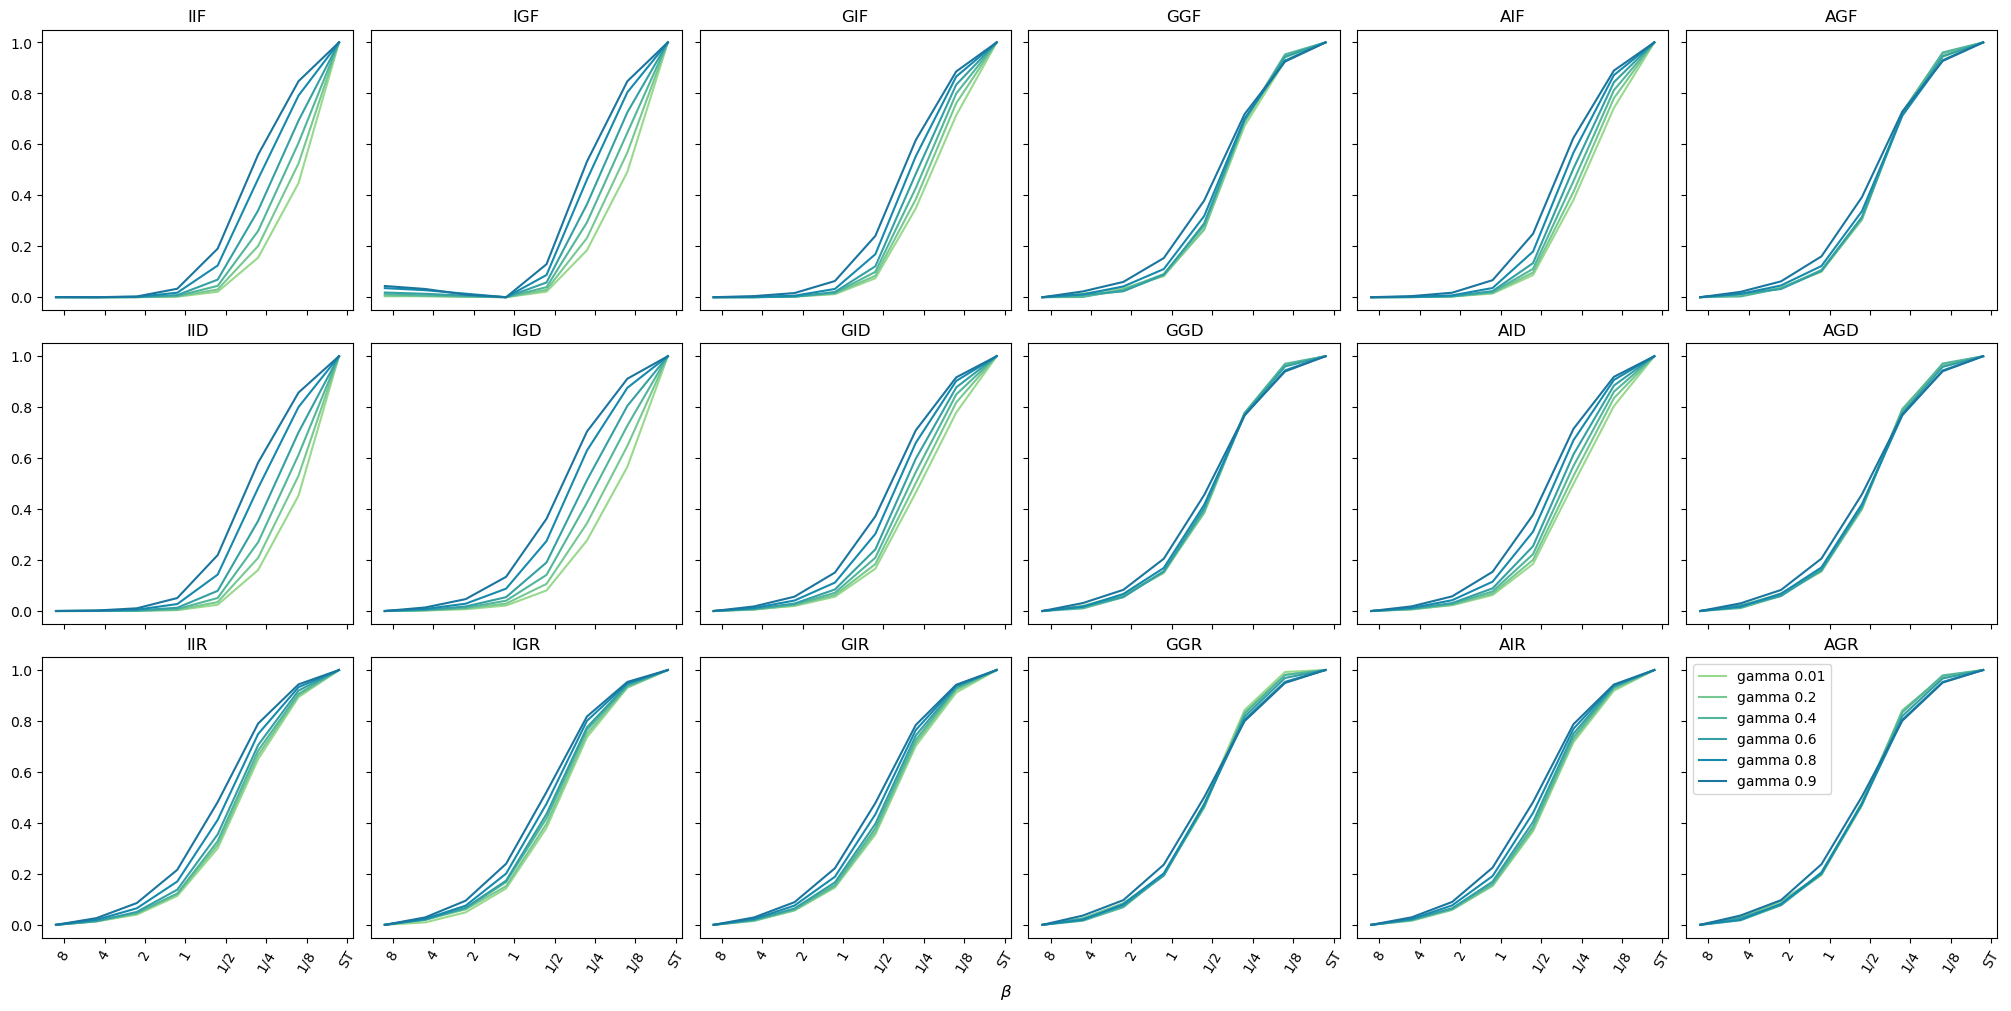
\includegraphics[width=\textwidth]{Figures/Figure_2_parametersweep.png}
        \caption{Group: Gender}
    \end{subfigure}
    \begin{subfigure}{\textwidth}
        \includegraphics[width=\textwidth]{Figures/Figure_2_parametersweep_age.png}
        \caption{Group: Age}
    \end{subfigure}
        \label{fig: param_fig2}
        \caption{Results for the Behavior of JME-fairness metrics for a stochastic ranking policy, using different values for gamma (patience factor). The same randomized BPRMF model is utilized as in figure \ref{fig: og_fig2}.}
\end{figure}

\begin{figure}[H]
    \centering
    \begin{subfigure}{\textwidth}
        \centering
        \includegraphics[width=1\textwidth]{Figures/Figure_3_parametersweep_gender.png}
        \caption{Group: Gender}
    \end{subfigure}
    \begin{subfigure}{\textwidth}
        \centering
        \includegraphics[width=1\textwidth]{Figures/Figure_3_parametersweep_age.png}
        \caption{Group: Age}
    \end{subfigure}
        \label{fig: param_fig3}
        \caption{Curves for disparity-relevance trade-off across the six different fairness dimensions for group 'Age', introducing different levels of stochasticity on top of the static rankings from the BPRMF model, initialized with six different gamma values.}
\end{figure}



\renewcommand{\thesubsection}{\textbf{\textcolor{black}{G}}}
\subsection{Computational Costs} \label{computation_costs}

\begin{center}
\begin{longtable}{|l|l|l|l|l|} 
\caption[Computational costs for running JME metrics]{Computational costs for running JME metrics} \\
\hline 
\multicolumn{1}{|c|}{\textbf{Model}} & \multicolumn{1}{c|}{\textbf{Dataset}} & \multicolumn{1}{c|}{\textbf{User Group Attr.}} & \multicolumn{1}{c|}{\textbf{Conduct}} & \multicolumn{1}{|c|}{\textbf{Time (s)}} \\ \hline
\endfirsthead

\multicolumn{3}{c}{{\bfseries \tablename\ \thetable{} -- continued from previous page}} \\ 
\multicolumn{3}{c}{} \\
\hline \multicolumn{1}{|c|}{\textbf{Model}} & \multicolumn{1}{c|}{\textbf{Dataset}} & \multicolumn{1}{c|}{\textbf{User Group Attr.}} & \multicolumn{1}{c|}{\textbf{Conduct}} & \multicolumn{1}{|c|}{\textbf{Time (s)}} \\ \hline
\endhead

\hline \multicolumn{3}{r}{{Continued on next page}} \\ 
\endfoot
\endlastfoot

BPRMF & ML-1M  & Gender & stochastic & 725.0684\\
BPRMF & ML-1M& Gender& static& 154.5441\\
BPRMF& ML-1M&Age&stochastic& 957.8651\\
BPRMF& ML-1M& Age& static& 180.7152\\
LDA& ML-1M& Gender& stochastic& 864.2498\\
LDA& ML-1M& Gender& static& 153.9465\\
LDA& ML-1M& Age& stochastic& 1089.0162\\
LDA& ML-1M& Age& static& 186.1006\\
PureSVD& ML-1M& Gender& stochastic& 715.7262\\
PureSVD& ML-1M& Gender& static& 151.7859\\
PureSVD& ML-1M& Age& stochastic& 950.048\\
PureSVD& ML-1M& Age& static& 188.2004\\
SLIM& ML-1M& Gender& stochastic& 719.0509\\
SLIM&ML-1M&Gender&static&151.7716\\
SLIM&ML-1M&Age&stochastic&956.7448\\
SLIM&ML-1M&Age&static&193.7132\\
WRMF&ML-1M&Gender&stochastic&741.1262\\
WRMF&ML-1M&Gender&static&161.2652\\
WRMF&ML-1M&Age&stochastic&993.4329\\
WRMF&ML-1M&Age&static&198.609\\
CHI2&ML-1M&Gender&stochastic&683.553\\
CHI2&ML-1M&Gender&static&161.7956\\
CHI2&ML-1M&Age&stochastic&935.251\\
CHI2&ML-1M&Age&static&197.9363\\
HT&ML-1M&Gender&stochastic&710.8722\\
HT&ML-1M&Gender&static&166.7169\\
HT&ML-1M&Age&stochastic&929.8073\\
HT&ML-1M&Age&static&199.2845\\
KLD&ML-1M&Gender&stochastic&692.9546\\
KLD&ML-1M&Gender&static&158.0465\\
KLD&ML-1M&Age&stochastic&932.6938\\
KLD&ML-1M&Age&static&192.4868\\
LMWI&ML-1M&Gender&stochastic&688.2506\\
LMWI&ML-1M&Gender&static&158.2718\\
LMWI&ML-1M&Age&stochastic&933.3253\\
LMWI&ML-1M&Age&static&192.1429\\
LMWU&ML-1M&Gender&stochastic&684.1796\\
LMWU&ML-1M&Gender&static&159.5841\\
LMWU&ML-1M&Age&stochastic&921.215\\
LMWU&ML-1M&Age&static&199.5242\\
SVD&ML-1M&Gender&stochastic&696.7073\\
SVD&ML-1M&Gender&static&164.047\\
SVD&ML-1M&Age&stochastic&942.2578\\
SVD&ML-1M&Age&static&198.7106\\
NNI&ML-1M&Gender&stochastic&686.0589\\
NNI&ML-1M&Gender&static&165.4972\\
NNI&ML-1M&Age&stochastic&932.6179\\
NNI&ML-1M&Age&static&199.6226\\
NNU&ML-1M&Gender&stochastic&688.285\\
NNU&ML-1M&Gender&static&162.959\\
NNU&ML-1M&Age&stochastic&938.2951\\
NNU&ML-1M&Age&static&197.7788\\
PLSA&ML-1M&Gender&stochastic&694.9885\\
PLSA&ML-1M&Gender&static&160.9721\\
PLSA&ML-1M&Age&stochastic&933.0947\\
PLSA&ML-1M&Age&static&198.9573\\
Random&ML-1M&Gender&stochastic&697.7134\\
Random&ML-1M&Gender&static&164.7631\\
Random&ML-1M&Age&stochastic&949.5797\\
Random&ML-1M&Age&static&200.4768\\
RM1&ML-1M&Gender&stochastic&690.9269\\
RM1&ML-1M&Gender&static&159.6506\\
RM1&ML-1M&Age&stochastic&943.9163\\
RM1&ML-1M&Age&static&199.4095\\
RM2&ML-1M&Gender&stochastic&686.7696\\
RM2&ML-1M&Gender&static&160.0639\\
RM2&ML-1M&Age&stochastic&929.7664\\
RM2&ML-1M&Age&static&194.2399\\
RSV&ML-1M&Gender&stochastic&686.5787\\
RSV&ML-1M&Gender&static&154.8014\\
RSV&ML-1M&Age&stochastic&924.8023\\
RSV&ML-1M&Age&static&190.9936\\
RW&ML-1M&Gender&stochastic&726.8647\\
RW&ML-1M&Gender&static&155.593\\
RW&ML-1M&Age&stochastic&986.0415\\
RW&ML-1M&Age&static&189.6771\\
UIR&ML-1M&Gender&stochastic&678.447\\
UIR&ML-1M&Gender&static&148.8541\\
UIR&ML-1M&Age&stochastic&935.432\\
UIR&ML-1M&Age&static&186.4008\\
Bert4Rec&ML-1M&Gender&static&261.659\\
Bert4Rec&ML-1M&Gender&stochastic&1779.0463\\
Bert4Rec&ML-1M&Age&static&330.8377\\
Bert4Rec&ML-1M&Age&stochastic&2256.4323\\      
\hline
\end{longtable}
\end{center}
